\section{Datasets and Distance Functions}
\label{sec:datasets-and-distance-functions}

Provide details on the datasets we use for benchmarks.

Add interesting t-SNE or UMAP embeddings of datasets.
For example~\ref{fig:discussion:umap-annthyroid-euclidean}

\begin{figure}[ht!]
    \centering
    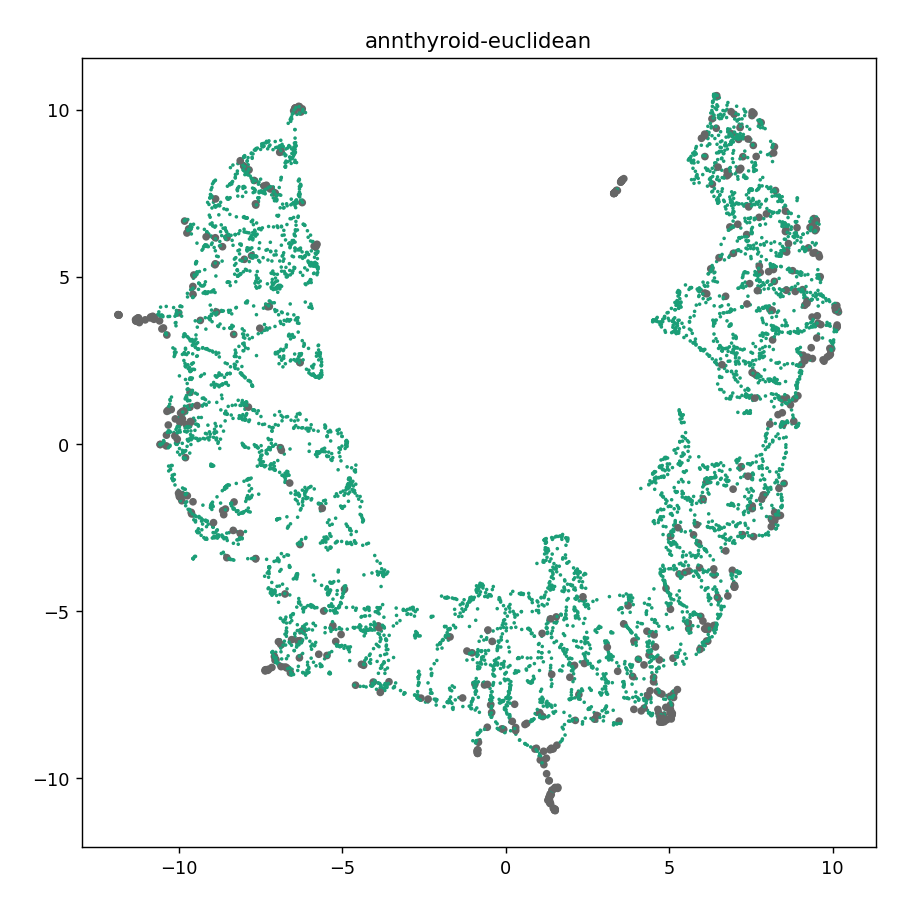
\includegraphics[width=2.5in]{images/umaps/annthyroid-euclidean-umap2d.png}
    \caption{UMAP embedding of Annthyroid data with the Euclidean distance function.}
    \label{fig:discussion:umap-annthyroid-euclidean}
\end{figure}

\subsection{APOGEE-2}
\label{subsec:datasets:apogee-2}

euclidean, cosine, wasserstein-1d

\dots

\subsection{MaNGA}
\label{subsec:datasets:manga}

euclidean, manhattan, wasserstein-2d

\dots

\subsection{Silva 18S and variants}
\label{subsec:datasets:silva-18s}

hamming, levenshtein

\dots

\subsection{ANN-Benchmarks suite}
\label{subsec:datasets:ann-benchmarks-suite}

deep1b: cosine

fashion-mnist: euclidean

gist: euclidean

glove: cosine

kosarak: jaccard

mnist: euclidean

nytimes: cosine

sift: euclidean

last.fm: cosine

\dots
